\chapter{APPLICATIONS TO IONIC SYSTEMS}
\label{ch:ionic_MgO}

In developing an interatomic potential, we define a database of properties (lattice parameter, cohesive energy, defect energies etc.) and their values for structures of interest. In fitting the potential, we have two priorities: first, to reproduce the values of the quantities in the fitting dataset as closely as possible; second, to ensure that the potential be robust, in that the predictions of the potential not be highly sensitive to small changes in the fitting database or the fitting procedure.

\begin{figure}[h]
	\centering
  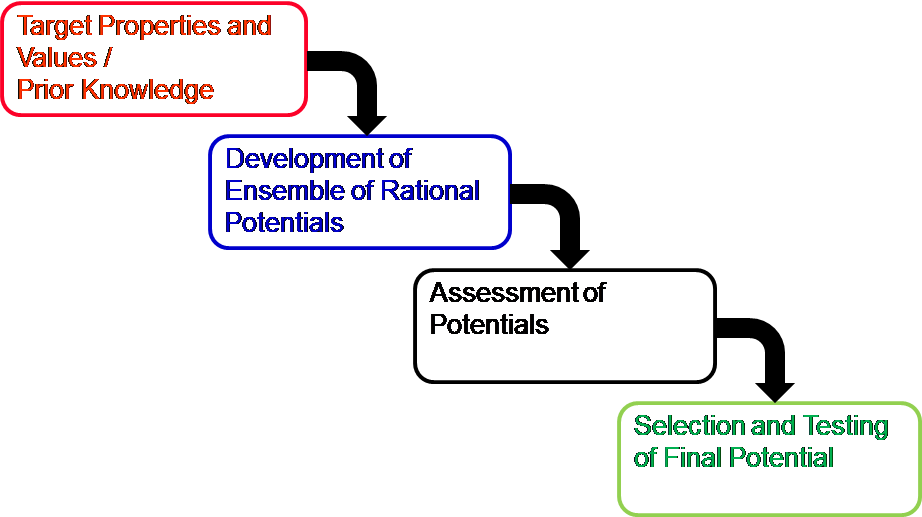
\includegraphics[width=0.8\textwidth]{chapter7/pareto_schematic}
  \caption{Schematic of the approach taken to potential development.}
  \label{fig:pareto_schematic}
\end{figure}

Figure \ref{fig:pareto_schematic} shows a schematic of the approach to the development of potentials outlined here. There are essentially four steps.
\begin{enumerate}
	\item The identification of structures, properties and their values to be used in the potential fitting. The specific values can be taken from experiment, from higher fidelity calculation methods such as quantum chemical or density functional theory (DFT) calculations, or a combination thereof. Our approach in this step is similar to standard potential development approaches.
 \item The use of ideas from Pareto optimization to develop an ensemble of rational potentials.  The concept of Pareto optimality was introduced discussed in Chapter \ref{ch:potential_development}. The term ‘rational’ will be discussed in detail below, but involves the use of a simple algorithm to identify potential parameterizations that make sense to consider further. This is the central idea of our approach and is very different from a conventional potential fitting approach
 	\item The analysis of the ensemble of rational potentials to identify features and clustering in both the high-dimensional parameter space and in the high-dimensional space of errors in the predictions of the properties.
 	\item The down-selection and testing of a few parameterizations or a single parameterization of the potential for use in further simulations.
\end{enumerate}

We focus mainly on the second of these steps: the development of an ensemble of rational potentials. We do, however, briefly discuss the other three parts of the process. For concreteness, we illustrate their use in the development of potentials for MgO, a simple and archetype ionic material.

As an illustration of the kind of information which can be obtained using a Pareto approach to parameterization and an example of the procedure shown in Fig. \ref{fig:pareto_schematic}, we consider the case of Buckingham potentials for magnesium oxide (MgO).

\section{Potential Formalism and Prior Knowledge}

Lewis and Catlow\cite{lewis1985_buckingham} parameterized a wide range of oxide systems with a pairwise potential, between two atoms $i$ and $j$.  In this formalism, the physics of an ionic system can be modelled with a pairwise Coulombic interaction between atoms $i$ and $j$, a short range repulsion due to the Pauli exclusion principle, and a van der Waals interaction term\cite{buckingham1938}

\begin{equation}
	V_{\alpha\beta}(r_{ij}) =
			\frac{Z_{\alpha}Z_{\beta}e^2}{r_{ij}}
			+ A_{\alpha\beta} \exp \left(\frac{r_{ij}}
																				{\rho_{\alpha\beta}}
															\right)
			- \frac{C_{\alpha\beta}}
			       {r_{ij}^6},
\end{equation}
with $\alpha$ and $\beta$ representing the chemical species of atoms $i$ and $j$, respectively.  The free parameters of the potential are $A_{\alpha\beta}$, $\rho_{\alpha\beta}$, and $C_{\alpha\beta}$ and $Z_i$.  The ionic charges which are allowed to deviate from their from their formal charges.  This information will be encoded as constraints to our optimization problem.

We examine three existing Buckingham potentials for MgO to define our initial vague (uninformed) estimate of the $p{\bm{\theta}}$ by assuming a uniform distribution on the domain of possible values of $p{\theta_i}$ defined by a lower and upper bound for each parameter $i$. Since MgO must be charge neutral, we restrict $Z_{\text{Mg}}= -Z_{\text{O}}$. For simplicity, and as is typical for Buckingham potentials, the Mg-Mg short-range interactions are set to zero ($A_\text{Mg-Mg}=0$ with $\rho_{\text{Mg-Mg}}=0.5$  for numerical stability), as is the van der Waals term for the Mg-O interaction ($C_{\text{Mg-O}}=0$). This leaves six free parameters in which to fit the potential (
$A_{\text{O-O}}$,
$\rho_{\text{O-O}}$,
$C_{\text{O-O}}$,
$A_{\text{Mg-O}}$,
$\rho_{\text{Mg-O}}$, and
$Z_{\text{Mg}}$).

In addition to the potential from Lewis and Catlow, two potentials unpublished Buckingham potentials were developed by Ball and Grimes (BG-2.0 and BG-1.7), but are available in the work of Henkelman \emph{et al.}\cite{henkelman2005_buckingham_MgO}.  For each parameter, we define the upper and lower bounds of the uninformative prior distribution from the three potentials in Table \ref{tlb:MgO_prior_potentials}, slightly increasing the range of values, as shown in Table \ref{tbl:MgO_inital_distribution}.

\begin{table}[ht]
	\caption{The Parameters for the empirical Buckingham potential for two formal charge potentials by Lewis and Catlow (LC)\cite{lewis1985_buckingham} and Ball and Grimes (BG-2.0). Another potential developed by Ball and Grimes (BG-1.7) uses partial charges. Parameters taken from Henkelman \emph{et al.}\cite{henkelman2005_buckingham_MgO}.}
	\label{tlb:MgO_prior_potentials}
	\centering
	\begin{tabular}{cccccc}
		\hline
		{Potential Name} & {$Z_{\text{Mg}}$ (e)} & Pair	 & $A$ (eV) & $\rho$ (\AA)	& $C$ ($\text{eV \AA}^6$) \\
		\hline
		LC	&    +2.00   &  Mg-O   &	 821.60  &   0.32000  &  0.00 \\
			  &            &   O-O	 & 22764.00	 &   0.14900  & 27.88 \\
		BG-2.0 & +2.00   &	Mg-O	 &  1279.69  &   0.29969  &  0.00 \\
		       &         & 	 O-O	 &  9547.96	 &   0.21916	& 32.00 \\
		BG-1.7 &  +1.70  &  Mg-O   &   929.69  &   0.29909  &	 0.00 \\
           &         &   O-O   &  4870.00	 &   0.26700  &	77.00 \\
		\hline
	\end{tabular}
\end{table}

\begin{table}[ht]
	\caption{Minimum and maximum values on the vague prior distribution for three parameters of the MgO Buckingham potential.}
	\label{tbl:MgO_inital_distribution}
	\centering
	\begin{tabular}{cccc}
    \hline
		$\theta_i$ & $\theta_i^{\text{MIN}}$ & $\theta_i^{\text{MAX}}$ & Units \\
		\hline
		$Z_{\text{Mg}}$ & +1.5 & +2.5 & e \\
		$A_{\text{Mg-O}}$ & +800.0 & +1300.0 & eV \\
		$rho_{\text{Mg-O}}$ & +0.2900 & +0.3300 & \AA \\
		$A_{\text{O-O}}$ & +500.0 & +2500.0 & eV \\
		$\rho_{\text{O-O}}$ & +0.1000 & +0.4000 & \AA \\
		$C_{\text{O-O}}$ & +25.00 & +75.00 & $\text{eV \AA}^6$ \\
	  \hline
	\end{tabular}
\end{table}

\subsection{Fitting Database}

We choose the target materials properties for MgO to be the lattice parameter, $a_0$, and elastic properties ($c_{11}$, $c_{12}$, $c_{44}$, and shear and bulk, $B$ and $G$) of the ground-state rock-salt (NaCl) structure, the \hkl(100) surface energy, the anion and cation Frenkel defect energies, and the Schottky defect formation energy.  Although $B$ and $G$ are fully determined by other elastic constants, it is useful to include them in the set of fitting database as they are the most physically accessible and measure the specific sums and differences in elastic properties that correspond to criteria for the stability of the crystal ($B > 0$, $G > 0$, $c_{44}> 0$).

Reference values for all of the targeted properties were calculated with VASP\cite{kresse1993_vasp,kresse1996_vasp1,kresse1996_vasp2} using the Perdew, Burke, and Ernzerhof generalized-gradient approximation (PBE-GGA) of the exchange-correlation functional \cite{perdew1996_gga_pbe}.
The lattice parameter and elastic properties were calculated from an 8-ion conventional cubic unit cell using a $6 \times 6 \times 6$ $k$-point mesh.  Surface energies were calculated using a $1 \times 1 \times 10$ supercell, with a slab thickness consisting of half of the height of the cell, and a $k$-point mesh of $9 \times 9 \times 1$.  Defect formation energies were calculated from $3 \times 3 \times 3$ supercells, using a $k$-point mesh of $3 \times 3 \times 3$.  The plane wave cutoff energy was set at $800$ eV. The resulting values of these quantities are showin in Table \ref{tbl:MgO_target} and constitute the QOIs for the parametrization process.

\begin{table}[ht]
	\caption[Target Properties of MgO]{Target properties of MgO and their values determined from DFT}
	\label{tbl:MgO_target}
	\centering
	\begin{tabular}{cccc}
		\hline
		 $q_i$ & Name & Units & {DFT (PBE-GGA)} \\
		\hline
    $q_1$ & $a_0$     & \AA   &	4.246 \\
    $q_2$ & $c_{11}$  & GPa   & 277.00 \\
    $q_3$ & $c_{12}$  & GPa   & 91.67 \\
    $q_4$ & $c_{44}$  & GPa 	& 144.01 \\
		$q_5$ & $B$       & GPa   & 153.45 \\
    $q_6$ & $G$       & GPa   & 92.66 \\
		$q_7$ & $E_{\text{fr,a}}$ & eV & 	10.978 \\
		$q_8$ & $E_{\text{fr,c}}$ & eV & 8.966 \\
		$q_9$ & $E_{\text{sch}}$ & eV &	5.067 \\
		$q_{10}$ & $\gamma_{\text{\hkl<100>}}$ & $\text{eV/\AA}^2$ &	0.056 \\
		\hline
	\end{tabular}
\end{table}

\section{Development of Ensemble of Rational Potentials}

With the identification of constraints and a fitting database determined, it is possible to define the parameterization problem.  Here, after choosing the loss function between predicted values $\hat{q}_i(\bm{\theta})$ and the target value $q_i$ with the absolute value function, $L_i(\bm{\theta})=|\hat{q}_i(\bm{\theta})-q_i|$ for each QOi $q$.q
\begin{align}
	&\min_{\bm{\theta}} &\bm{L}(\bm{\theta})=[
	    L_1(\bm{\theta}),
			L_2(\bm{\theta}),
			...,
			L_9(\bm{\theta})] \\
	&\text{subject to} &g_1: Z_{\text{Mg}} > 0.0 \\
	& &g_2: A_{\text{Mg-O}} > 0.0 \\
	& &g_3: \rho_{\text{Mg-O}} > 0.0 \\
	& &g_4: A_{\text{O-O}} > 0.0 \\
	& &g_5: \rho_{\text{O-O}} > 0.0 \\
	& &g_6: C_{\text{O-O}} < 0.0 \\
	& &g_7: B > 0 \\
	& &g_8: G > 0 \\
	& &g_9: c_{44} > 0 \\
  & &h_1: Z_{\text{O}} = -Z_{\text{Mg}} \\
  & &h_2: A_{\text{Mg-Mg}} = 0.0 \\
  & &h_3: \rho_{\text{Mg-Mg}} = 0.5 \\
	& &h_5: C_{\text{Mg-O}} = 0.0 \\
  & &h_4: C_{\text{Mg-Mg}} = 0.0
\end{align}
where $g_i$ are inequality constraints and $h_i$ are equality constraints.

The machine-learning process of the generation of parameter sets, simulation management, and parallelization are provided through software developed in Python and MPI, as discussed in Chapter \ref{ch:software}. The energy calculations are performed using the LAMMPS\cite{plimpton1995_lammps} code. Long-range Coulombic interactions are computed in LAMMPS using the particle-particle mesh\cite{hockney1988_ppm}.  The entire autonomous workflow was illustrated in Figure \ref{fig:pareto_optimization}. The random generation of parameters sometimes results in an unusable potential (e.g. a failure in structural minimization); these parameters (less than 10\% of those tried) are discarded and are not included among the final 10,000 parameterizations.
Sampling from the vague distributions defined above, we generate N=10,000 sample potential parameterizations. The Pareto points are identified by removing the dominated points; This results in a Pareto set of  $N_\text{pareto} = 955$ potentials that provide a first estimate of the six-dimensional Pareto surface. We use the distribution of parameters in this Pareto set to provide a better estimate of the distribution functions of the parameters.  While an empirical discrete non-parametric probability distribution function can be calculated from the histogram of parameters of the Pareto optimal potentials, it is preferable to sample a random variable defined by a smooth, and continuous probability distribution function. The kernel density estimation (KDE) provides a parameter-free estimate of the probability density functions\cite{rosenblatt1956_kde,parzen1962_kde} and provides the ability to uncover features in the estimate of probability density function which are not apparent in the histogram. If we assume each member of the Pareto set to be independent and identically distributed from some distribution with unknown density $p_{\Theta^*}$, we can the estimate of the shape of $p(\bm{\theta}^*)$, which we now define exactly.
Let $\bm{\theta}_{t-1,1}^*,...,\bm{\theta}_{t-1,N}^*$ be $N$ samples of $N_P$-dimensional parameter sets belonging to the Pareto set from the previous iteration, $t-1$, be described by the density function $\hat{p}_{\bm{\Theta}}(\bm{\theta}_t)$.  The multivariate kernel density estimate is defined to be
\begin{equation}
	\hat{f}_{\bm{\Theta}_t}(\bm{\theta}|\bm{H})
			= \frac{1}{N}\sum_{i=1}{N}\bm{K}_{\bm{H}}(\bm{\theta}-\bm{\theta}_i)
\end{equation}
where $\bm{K}_{\bm{H}} = |\bm{H}|^{-1/2} K ({\bm{H}}^{-1/2}\bm{\theta})$ with $K$ being a kernel function which is has a symmetric multivariate density, $\bm{H}\in \mathbb{R}^{N_P\times N_P}$ is bandwidth matrix which is symmetric and postive definite.  Since the choice of the kernel function is not critical to the accuracy of kernel density estimators in most cases\cite{wand1995_kde}, the Gaussian kernel is chosen.  Then $\bm{H}$ is the bandwidth matrix which affects the direction and orientation of smoothing induced.
Here, $\bm{H}$ is determined from the covariance matrix for the parameter matrix from the previous iteration is used $\bm{\Theta}_{t-1}$, and modified by a scaling factor determined by the Silverman method\cite{silverman1986_kde}, which minimizes the mean integrated square differences.

Figure \ref{fig:Z_Mg_iter_0} illustrates the distribution of the ionic charge of Mg ions, $Z_{\text{Mg}}$, after sampling from the uniform distribution.  Since $Z_{\text{Mg}}$ is initially sampled from a uniform distribution, the histogram indicates the strict discontinuous limits of the lower and upper bounds of the distribution.  The coarse-grained nature of the discrete bins in the histogram would make it difficult to identify the most probable values of $Z_{\text{Mg}}$ or even the departure of the Pareto set population from the original uniform distribution from which $Z_{Mg}$ is generated.  Attempting to use the normal distribution from the sample mean and variance does not capture the underlying features of the uniform.  However, the KDE is able to estimate the underlying probability distribution function with some distortion at the upper and lower bounds due to exponential tails of the Gaussian distribution.

\begin{figure}[ht]
	\centering
  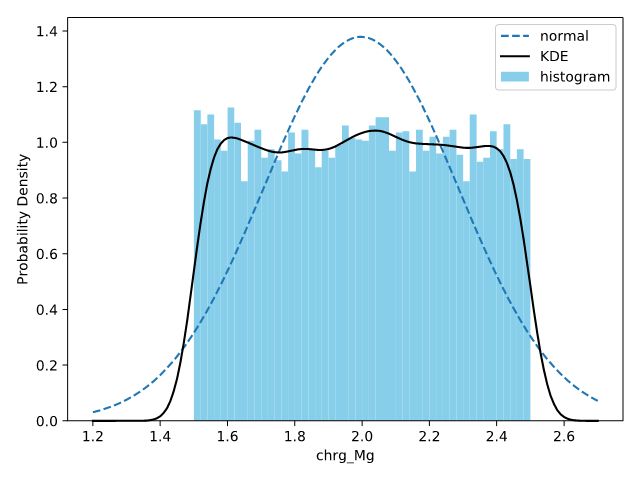
\includegraphics[width=0.8\textwidth]{chapter7/Z_Mg_iter_0}
  \caption{The distribution of the parameter which controls the partial charge distribution of the magnesium ion, $Z_{\text{Mg}}$, in the Pareto set. The histogram of which is a discrete representation of the distribution of $Z_{\text{Mg}}$, continuous distributions of the distribution of $Z_{\text{Mg}}$ is estimated by the kernel density estimate.}
  \label{fig:Z_Mg_iter_0}
\end{figure}

Figure \ref{fig:Z_Mg_iter_0_pareto} illustrates the changes in the KDE as it goes through sampling, Pareto-optimality filtering, and performance filtering.  The blue dashed line shows the distribution in charge for all points sampled. When the dominated parameterizations are removed from the set to determine the Pareto set, the KDE (orange dashed line) indicates a concentration of parameterizations in the region $Z_{\text{Mg}} \approx +1.8 \text{e}$.  Next, we cull the Pareto set by removing the largest outliers by percentile, determined by $|\hat{q}_i -q_i|$.  This eliminates $2$\% of pathological parameterizations which are Pareto efficient; this results in the green dashed line in Figure \ref{fig:Z_Mg_iter_0_pareto}.

\begin{figure}[ht]
	\centering
  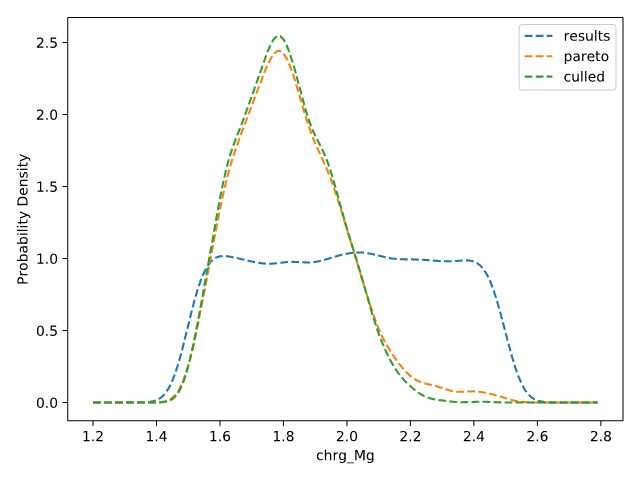
\includegraphics[width=0.8\textwidth]{chapter7/Z_Mg_iter_0_pareto}
  \caption{A single variable visualization of the population of parameterization for the charge parameter, $Z_{\text{Mg}}$ after the first iteration}
  \label{fig:Z_Mg_iter_0_pareto}
\end{figure}

Ten iterative improvements are made to estimate the Pareto surface using updates to the KDE probability distribution described earlier using the Silverman selection of the smoothing parameter. The evolution of the set of solutions comes from the refinement of the probability density function which represents the set of solutions.  In the initial iteration (N=0), the probabiity distribution resembles a uniform distribution.  The probability distribution evolves rapidly to a triangular shaped probability distribution made smooth by the KDE Gaussian tails, but the resolution of the region of maximum likelihood (the peak of the density function does not happen until $N=9$

\begin{figure}[ht]
	\centering
  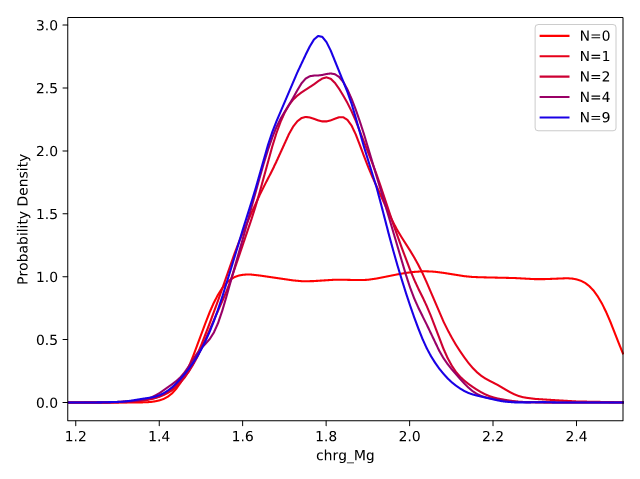
\includegraphics[width=0.8\textwidth]{chapter7/Z_Mg_evolution}
  \caption{Evolution of the predicted charge parameter $Z_{\text{Mg}}$.  These curves are the univariate probability distribution function, using the Silverman method for determining the smoothing parameter.}
  \label{fig:Z_Mg_evolution}
\end{figure}

Since the number of materials properties constitutes a high-dimensional space, analysis of the Pareto surface is most conveniently performed in a series of bi-objective scatter plots which project, or slice, the error-space information onto the the 2D space.  A representative improvement of the Pareto surface estimate is shown in Figure \ref{fig:MgO_biobjective_evolution}, which shows the first four iterations of Pareto estimation process by looking at,
$|\epsilon_i(\bm{\theta})=|\hat{q}_i(\bm{\theta})-q_i|$, $\bm{\theta}\in\bm{\Theta}_t^*$ for the bulk modulus ($B$) and the lattice parameter ($a_0$).  This bivariate plot projects the $N_Q$ dimensional $\epsilon$-space is projected onto tje two-dimensional $\epsilon$-space for $B$ and $a_0$. In the initial iteration, the uniformative distribution selects a range of parameter which have large errors.  In subsequent iterations, the KDE predicts parameterizations in the neighborhood of previously found Pareto optimal points resulting in $q(\bm{\theta})$ being clustered closer to the origin.   The KDE is explictly chosen because for the ability to capture departures from the multivariate-normal distribution.  There are points close to the origin in this-two dimesional project of the Pareto surface; however, these points do not have small errors in the other properties.

\begin{figure}[ht]
	\centering
  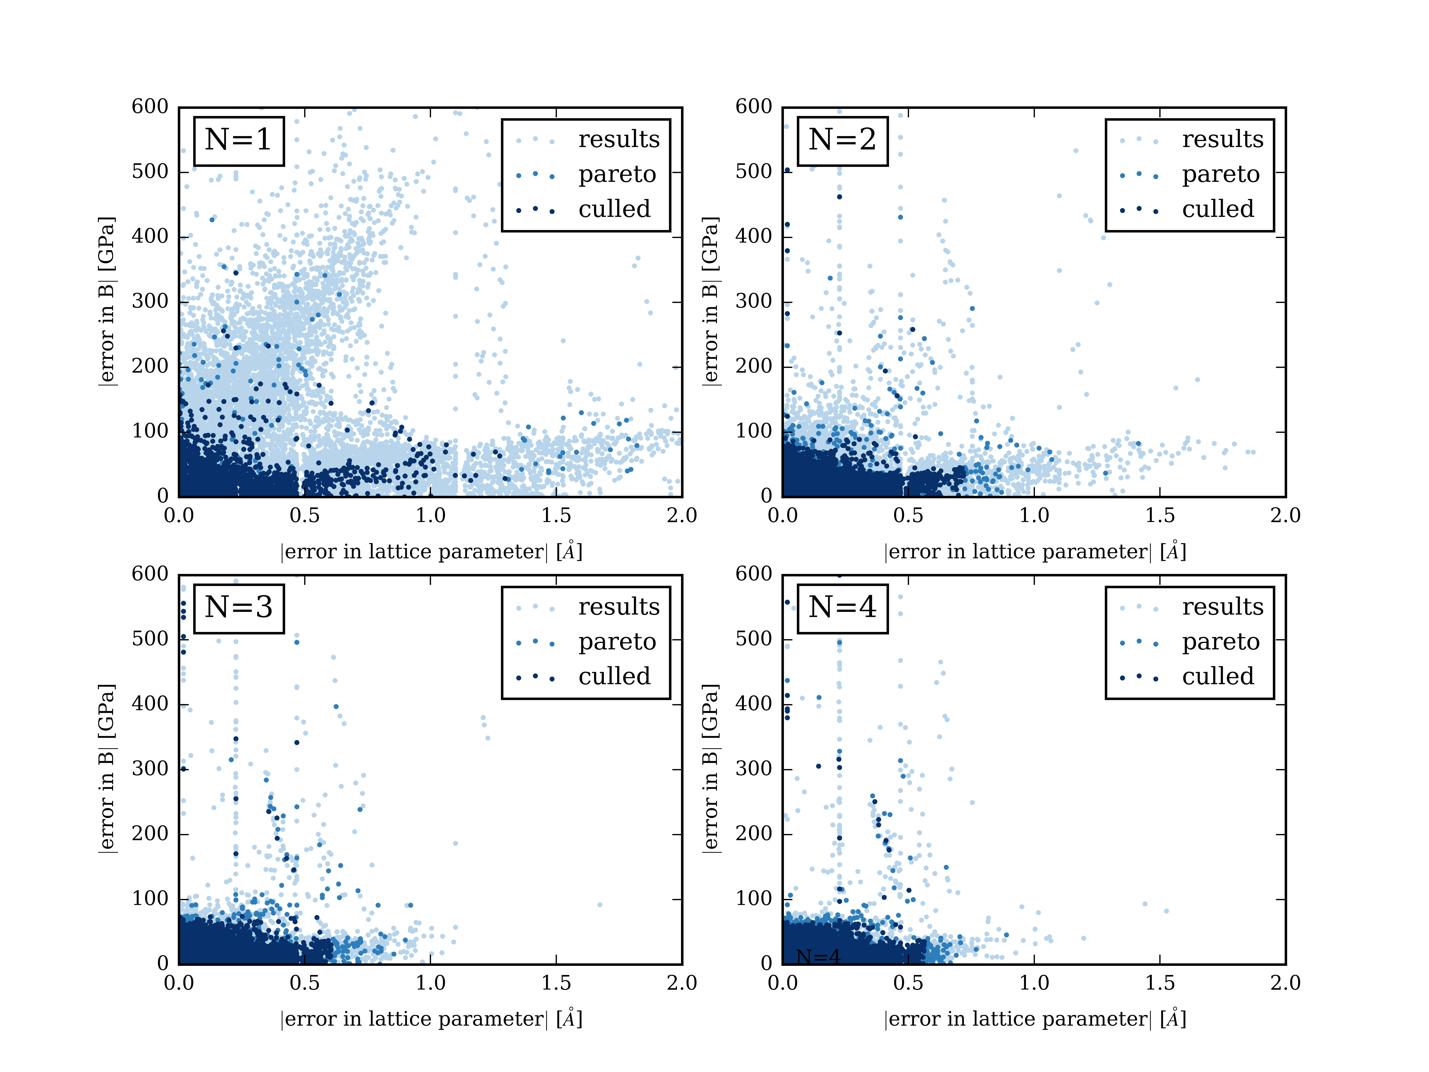
\includegraphics[width=0.8\textwidth]{chapter7/MgO_biobjective_evolution}
  \caption{Evolution of the predicted charge parameter $Z_{\text{Mg}}$.  These curves are the univariate probability distribution function, using the Silverman method for determining the smoothing parameter.}
  \label{fig:MgO_biobjective_evolution}
\end{figure}

In a multivariate-normal distribution, the correlation between parameters may be significant, and is captured in the variance-covariance matrix. This allows for more sophisticated analysis and refinement of the distribution functions. For example, the relationship between the parameters $A_{\text{O-O}}$ and $\rho_{\text{O-O}}$ are captured in Figure \ref{fig:MgO_biobjective_A_v_rho_OO}.  A visual inspection of the data shows a negative correlations between the two terms; as $A_{\text{O-O}}$ increases  $\rho_{\text{O-O}}$ tends to decrease.  This relationship is not surprising since these two quantities both parameterize the exponential repulsion, for which an increase in the decay length, $\rho$, can be compensated for by a decrese in the prefactor, $A$, and vice versa.

\begin{figure}[ht]
	\centering
  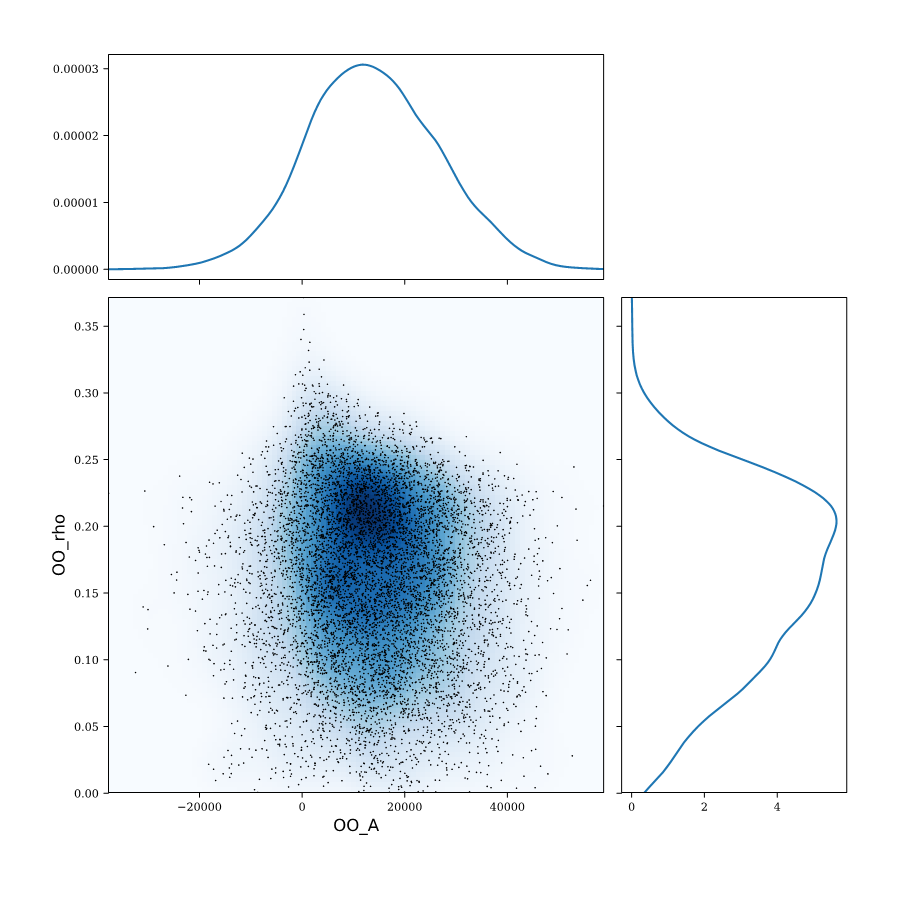
\includegraphics[width=0.8\textwidth]{chapter7/MgO_biobjective_A_v_rho_OO}
  \caption{Probability density functions and joint probability density functions of the KDE representing set of solutions for parameters $A_{\text{O-O}}$ and $\rho_{\text{O-O}}$.  The main figure is the joint probability density function with darker values being higher probability regions.  The vertical and horizontal probability density functions.}
  \label{fig:MgO_biobjective_A_v_rho_OO}
\end{figure}

When this iterative process is complete, we have an ensemble of $N=7557$ Pareto efficient MgO Buckingham potentials and associated potential parameters.

To this point in the process, unlike the gradient method, the potential developer has not provided any information as to their preferences in terms of acceptable errors or weights. Rather, the process has been an objective analysis of the capablities of the potential form to reproduce the targeted materials properties.  Thus, this process is complectely algorithmic in that for the potential form and target values, another developer should produce a statisitcially identical ensemble of Pareto optimial potentials. Further, if the the vague prior, iteration sequence and random numbers used in the sampling are defined, another developer should reproduce exactly the same ensemble of potentials.

An iterative procss can continue indefintiely. Thus, we need to establish criterea for satisfactory convergence. In deterministic methods, the numerical refinement is halted by a convergence condition, where the numerical solution changes slow as the optimal solution is approached.  The solutions to a multi-objective problem are a set of solutions.  Our solution method represents the set of solutions as a probability density function, which are estimated from the \emph{Pareto set}, the parameterizations which produce the Pareto surface in objective space, $\bm{\Theta}_i^*$, for the $i$th iteration.  A statistical analog to numerical convergence is to assess the convergence of the distribution, where we look at the difference of the distribution of the samples as a measure of convergence. The Kullback-Liebler\cite{kullback1951_kld} divergence, $D_{\text{KL}}(f_1 \vert f_2)$, measures how one probability distribution, $f_1$, diverges from a second probability distribution function, $f_2$.  For continuous random variables, $D_{\text{KL}}$, is defined as the integral
\begin{equation}\label{eq:kld}
    D_{\text{KL}} - \int f_1(x) \log \frac{f_1(x)}{f_2(x)} dx
\end{equation}
$D_{\text{KL}} \geq 0$, with $D_{\text{KL}} (f_1 \vert f_2 )=0$, when $f_1$=$f_2$, almost everywhere.  For our application, our distributions are KDEs, so the evaluation of the integral can be done by Monte Carlo integration\cite{hershey_kld_mc_integration}.  As the number of iterations, $i$, increases, the Kullbach-Liebler divergence $D_{\text{KL}}(f_{i-1}\vert f_i )$, converges asymtotically to $0$.

Since early iterations are more likely to cause changes in the set approximating $\bm{\Theta}^*$ than later simulations, changes in $D_{\text{KL}}$ will initially be large.  However, it becomes increasingly more difficult to identify further Pareto optimal solutions later in the simulation.  As a result, the distribution becomes more stationary.  However, since this integral is evaluated by Monte Carlo estimation, the KDE estimate of the distributions from the sample population will have small divergences betweem, $f_i(\bm{\theta}) and f_{i-1}(\bm{\theta})$, even if the KDE is the same distribution function.

Even 2D views of the Pareto set can identify shortcomings with potential formalisms.  The bi-objective plot in Figure \ref{fig:MgO_bivariate_c11_v_c44}, a slice through the data rather than projection of all of the data, illustrates a well-known limitation with the form of the Buckingham potential: there is a strong relationship between the $c_{11}$ and the $c_{44}$ of the elastic tensor, making reduction in the error of one lead to an increase in error in the other.

\begin{figure}[ht]
	\centering
  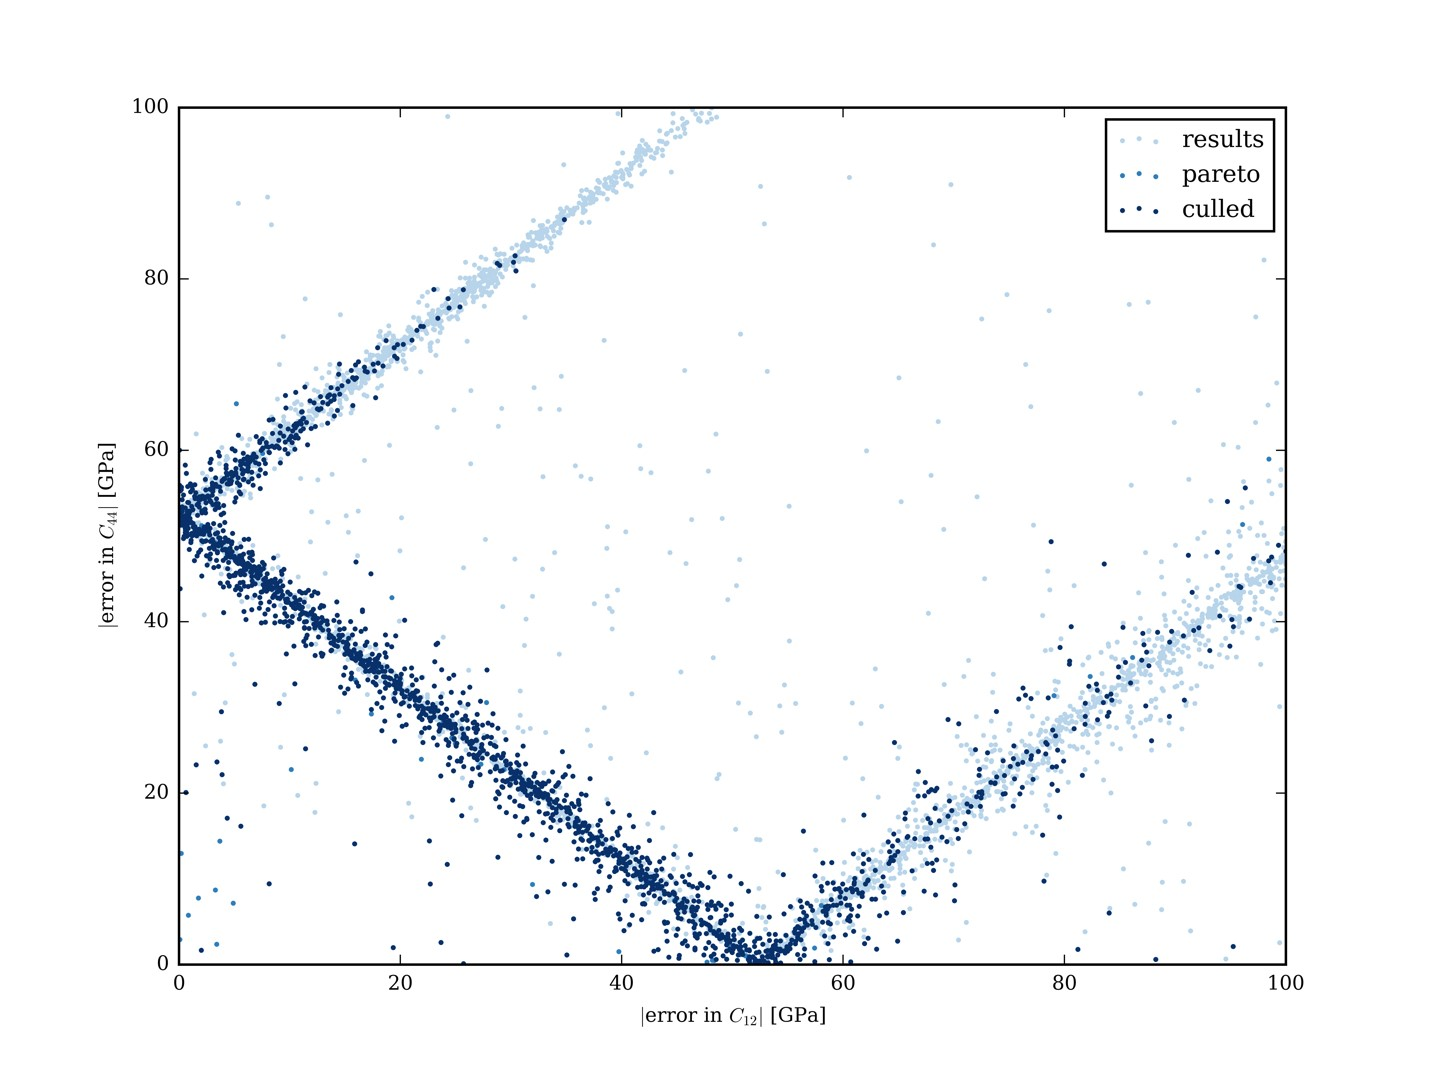
\includegraphics[width=0.8\textwidth]{chapter7/MgO_bivariate_c11_v_c44}
  \caption{Projection of the Pareto surface  in $\epsilon$-space projected onto the $|\epsilon_{c_{12}}|$ and $|\epsilon_{c_{44}}|$ subspace.  The 2D slice of data identifies a key tradeoff of the Buckingham potential.}
  \label{fig:MgO_bivariate_c11_v_c44}
\end{figure}


\section{Assessment of Potentials and Selection of Final Potentials}

Having generated an ensemble of Pareto-optimized potentials, the challenge now lies in down-selecting to a final set potentials for testing and full evaluation. The analysis performed to this point has been essentially algorithmic. For a specific formalism and specific material, the only input provided by the developer has been the properties to be considered in the fitting and their target values. Notably absent in the analysis to this point has been any statement of the acceptable errors in any of the targeted properties or any weighting factors. Rather, the analysis purely characterizes the capabilities of the potential. The result has been the Pareto optimal ensemble of interatomic potentials, any one of which is a rational choice in the sense of minimizing the errors. For an MD simulation, it is necessary to use a single potential; that is the developer must select one of the hundreds or thousands of rational choices coming from the Pareto analysis.  It thus at this stage of the process that the developer introduced their preferences into the analysis, thereby enabling the down-selection process.

	There are numerous ways of going about this process; unlike the construction of the Pareto ensemble, it is not uniquely defined.  As an illustration of one simple approach, we begin by normalizing the errors, $\epsilon_i$, by the target value, $q_i$; these normalized errors are now all dimensionless and are typically of order unity.  The 10 potentials closest to the origin, defined as the unweighted normalized sum of the squared scaled errors, are selected for further analysis.  In Figure \ref{fig:MgO_qoi_rugplots}, the performances of these $10$ Pareto-efficient potentials (black lines) are compared to potentials of Lewis-Catlow (green), Ball-Grimes±2.0 (blue), and Ball-Grimes±1.7 (red) potentials with respect to target values in Table \ref{tbl:MgO_target}. It is clear that the Pareto efficient potentials result in lower errors in the predicted values of almost all target physical quantities as compared to the expertly-determined reference potentials.

Having down-selected to 10 potentials, it is important to test their performances for properties that are not included in the fitting process. We calculate materials properties for quantities which are not part of the training set.  Specifically, we calculate the frequency of the zone-center optical phonon frequency for MgO, and the linear thermal expansion coefficient.  The phonon calculations are evaluated for the primitive cell of the rocksalt structure using GULP\cite{gale2003_gulp}.  The thermal expansion is determined from MD simulations. These results are compared from DFT-GGA calculations in the case of phonons ($385 \text{cm}^{-1})$, and from experimental data ($1.08\times10^{-5}$ \\A/\degree C) \cite{ho1998_thermal_expansion} in the case of thermal expansion.

\begin{figure}[ht]
	\centering
  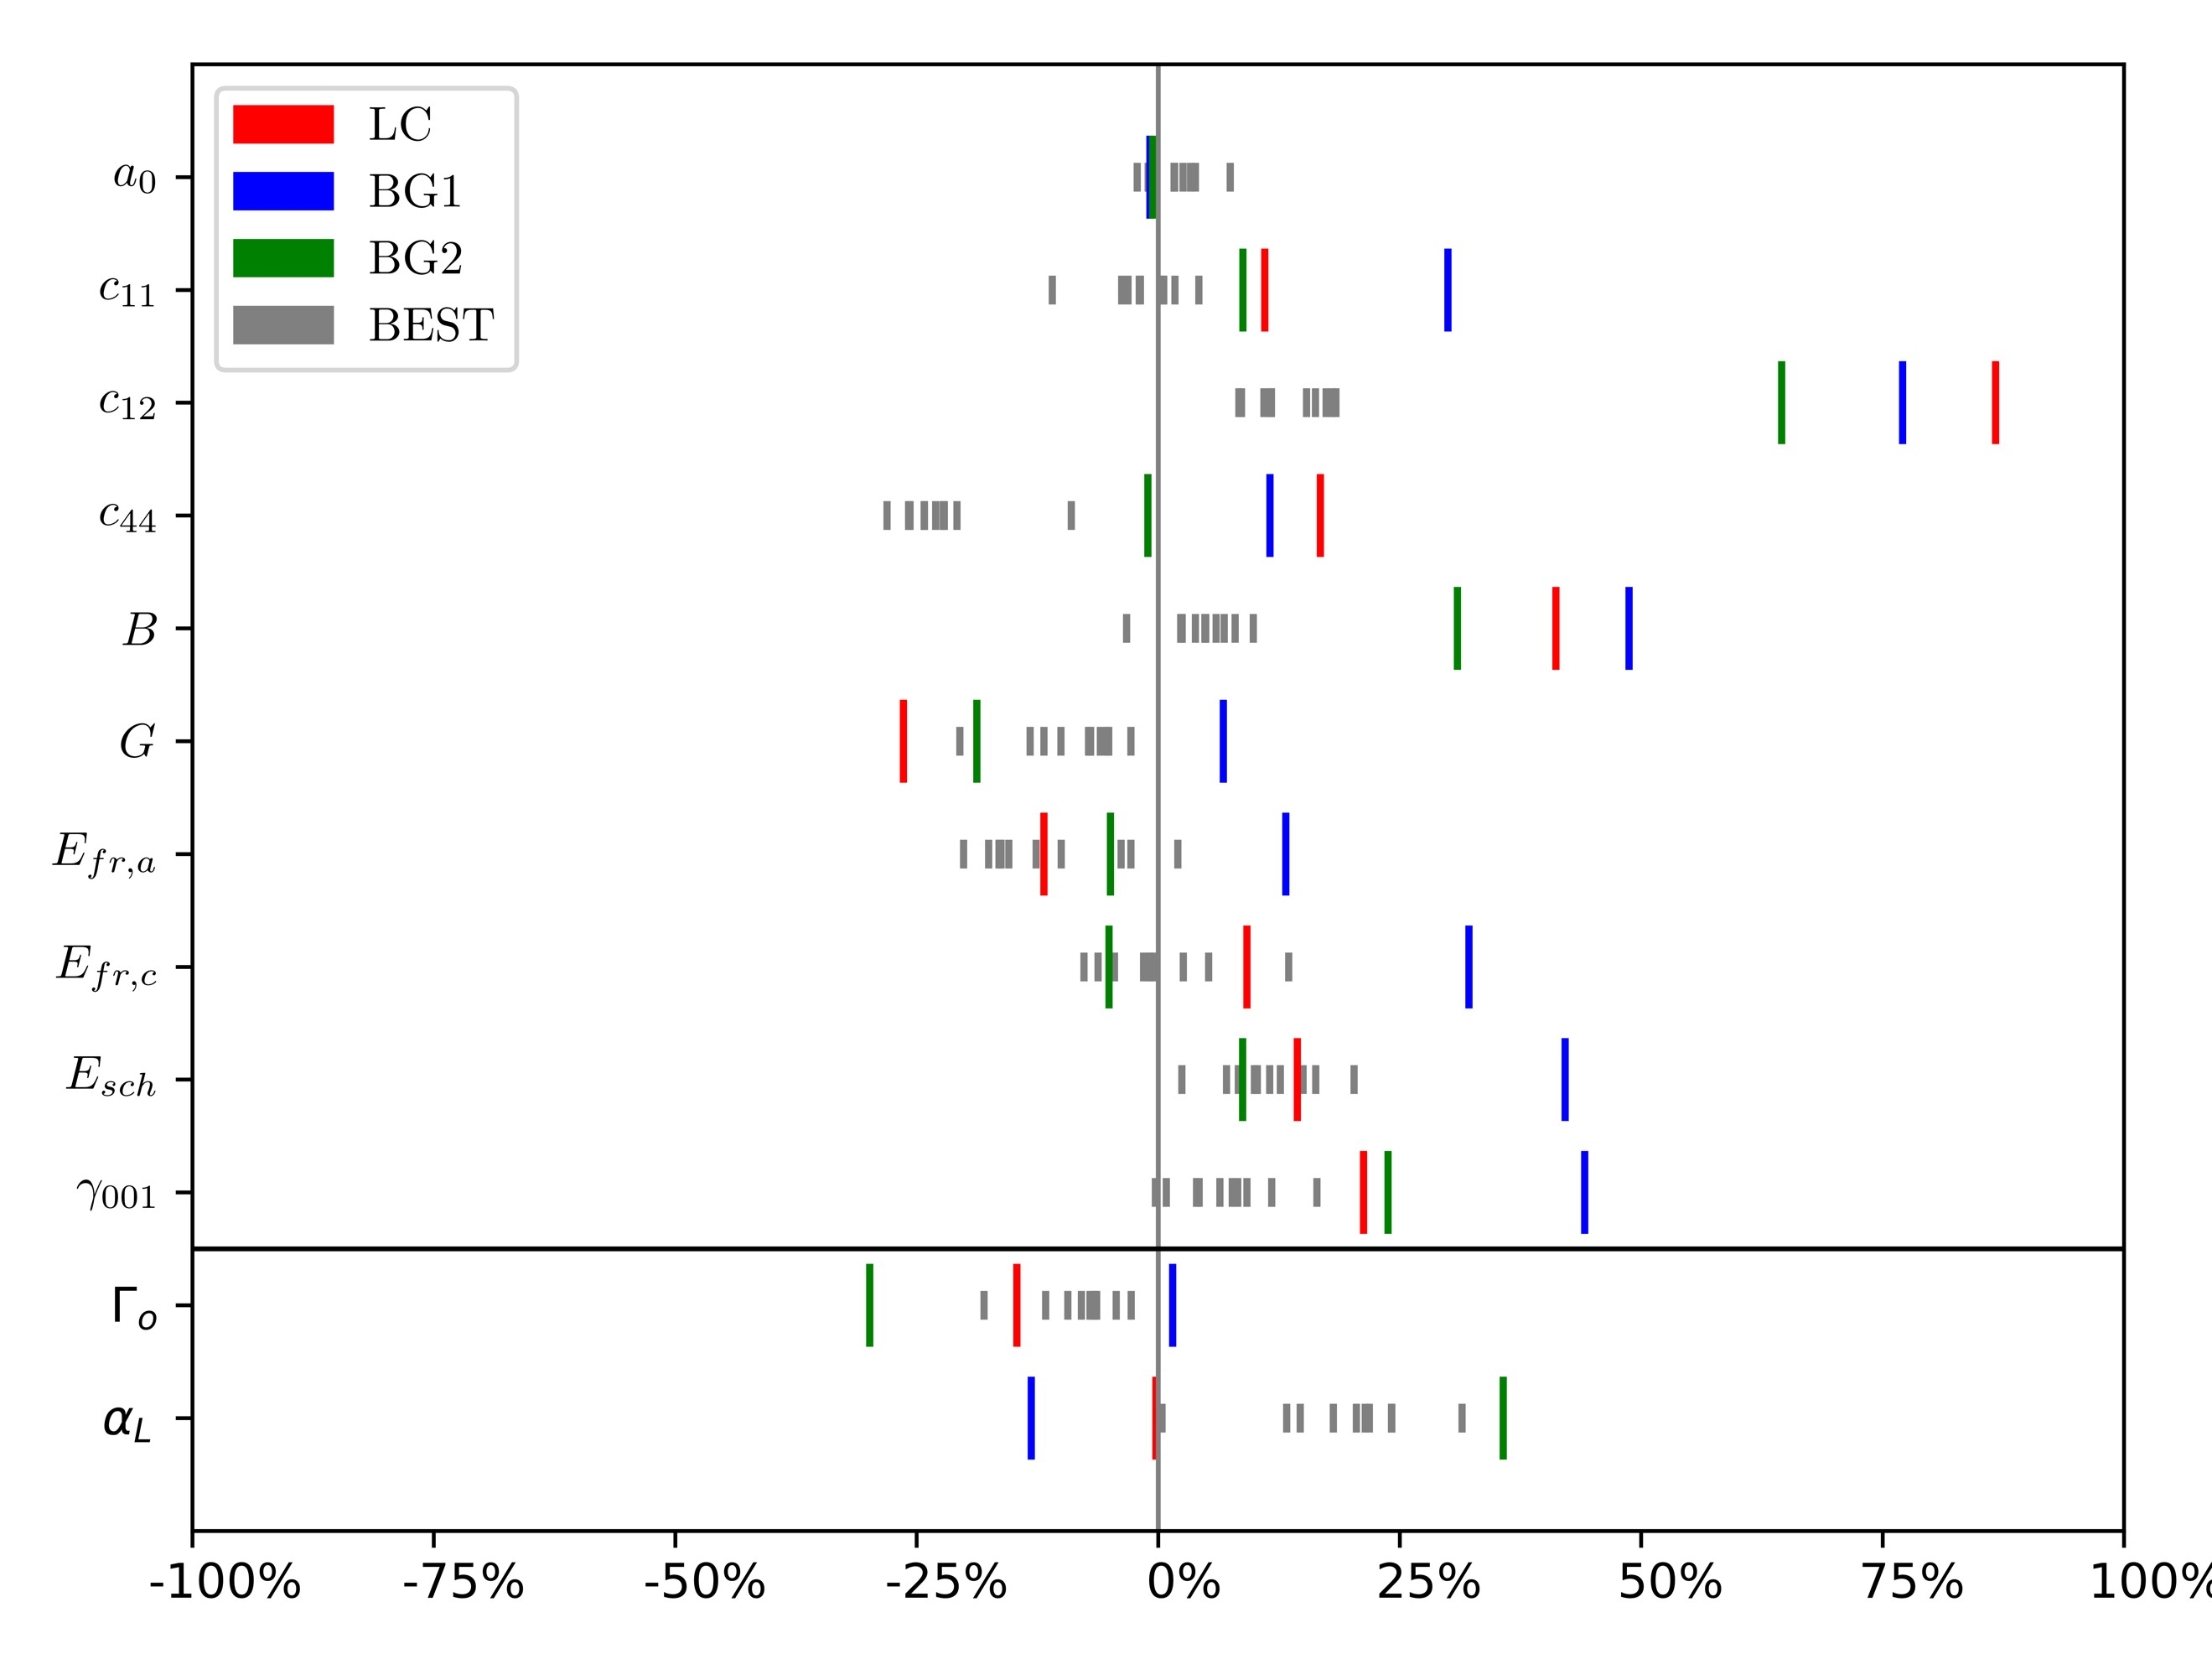
\includegraphics[width=0.8\textwidth]{chapter7/MgO_qoi_rugplots}
  \caption{Comparison of the errors in target quantities for 10 Pareto efficient parameterizations (black bars) of the Buckingham potential for MgO with predictions of three expert-developed potentials. The reference values are from the DFT calculations.}
  \label{fig:MgO_qoi_rugplots}
\end{figure}


To characterize this further, Figure \ref{fig:MgO_qoi_parallel_plots} compares the 10 best potentials selected in the way defined above to the LC, BG-2.0 and BG-1.7 potentials. Again, it is clear that in general, the potentials determined in this autonomous, machine-learning approach provide as high materials fidelity as the expert-developed potentials. The parameters and property values for these 10 best potentials and the three expert-developed potentials are shown in Tables \ref{tbl:MgO_best_param} and \ref{tbl:MgO_best_qoi}.

\begin{figure}[ht]
	\centering
  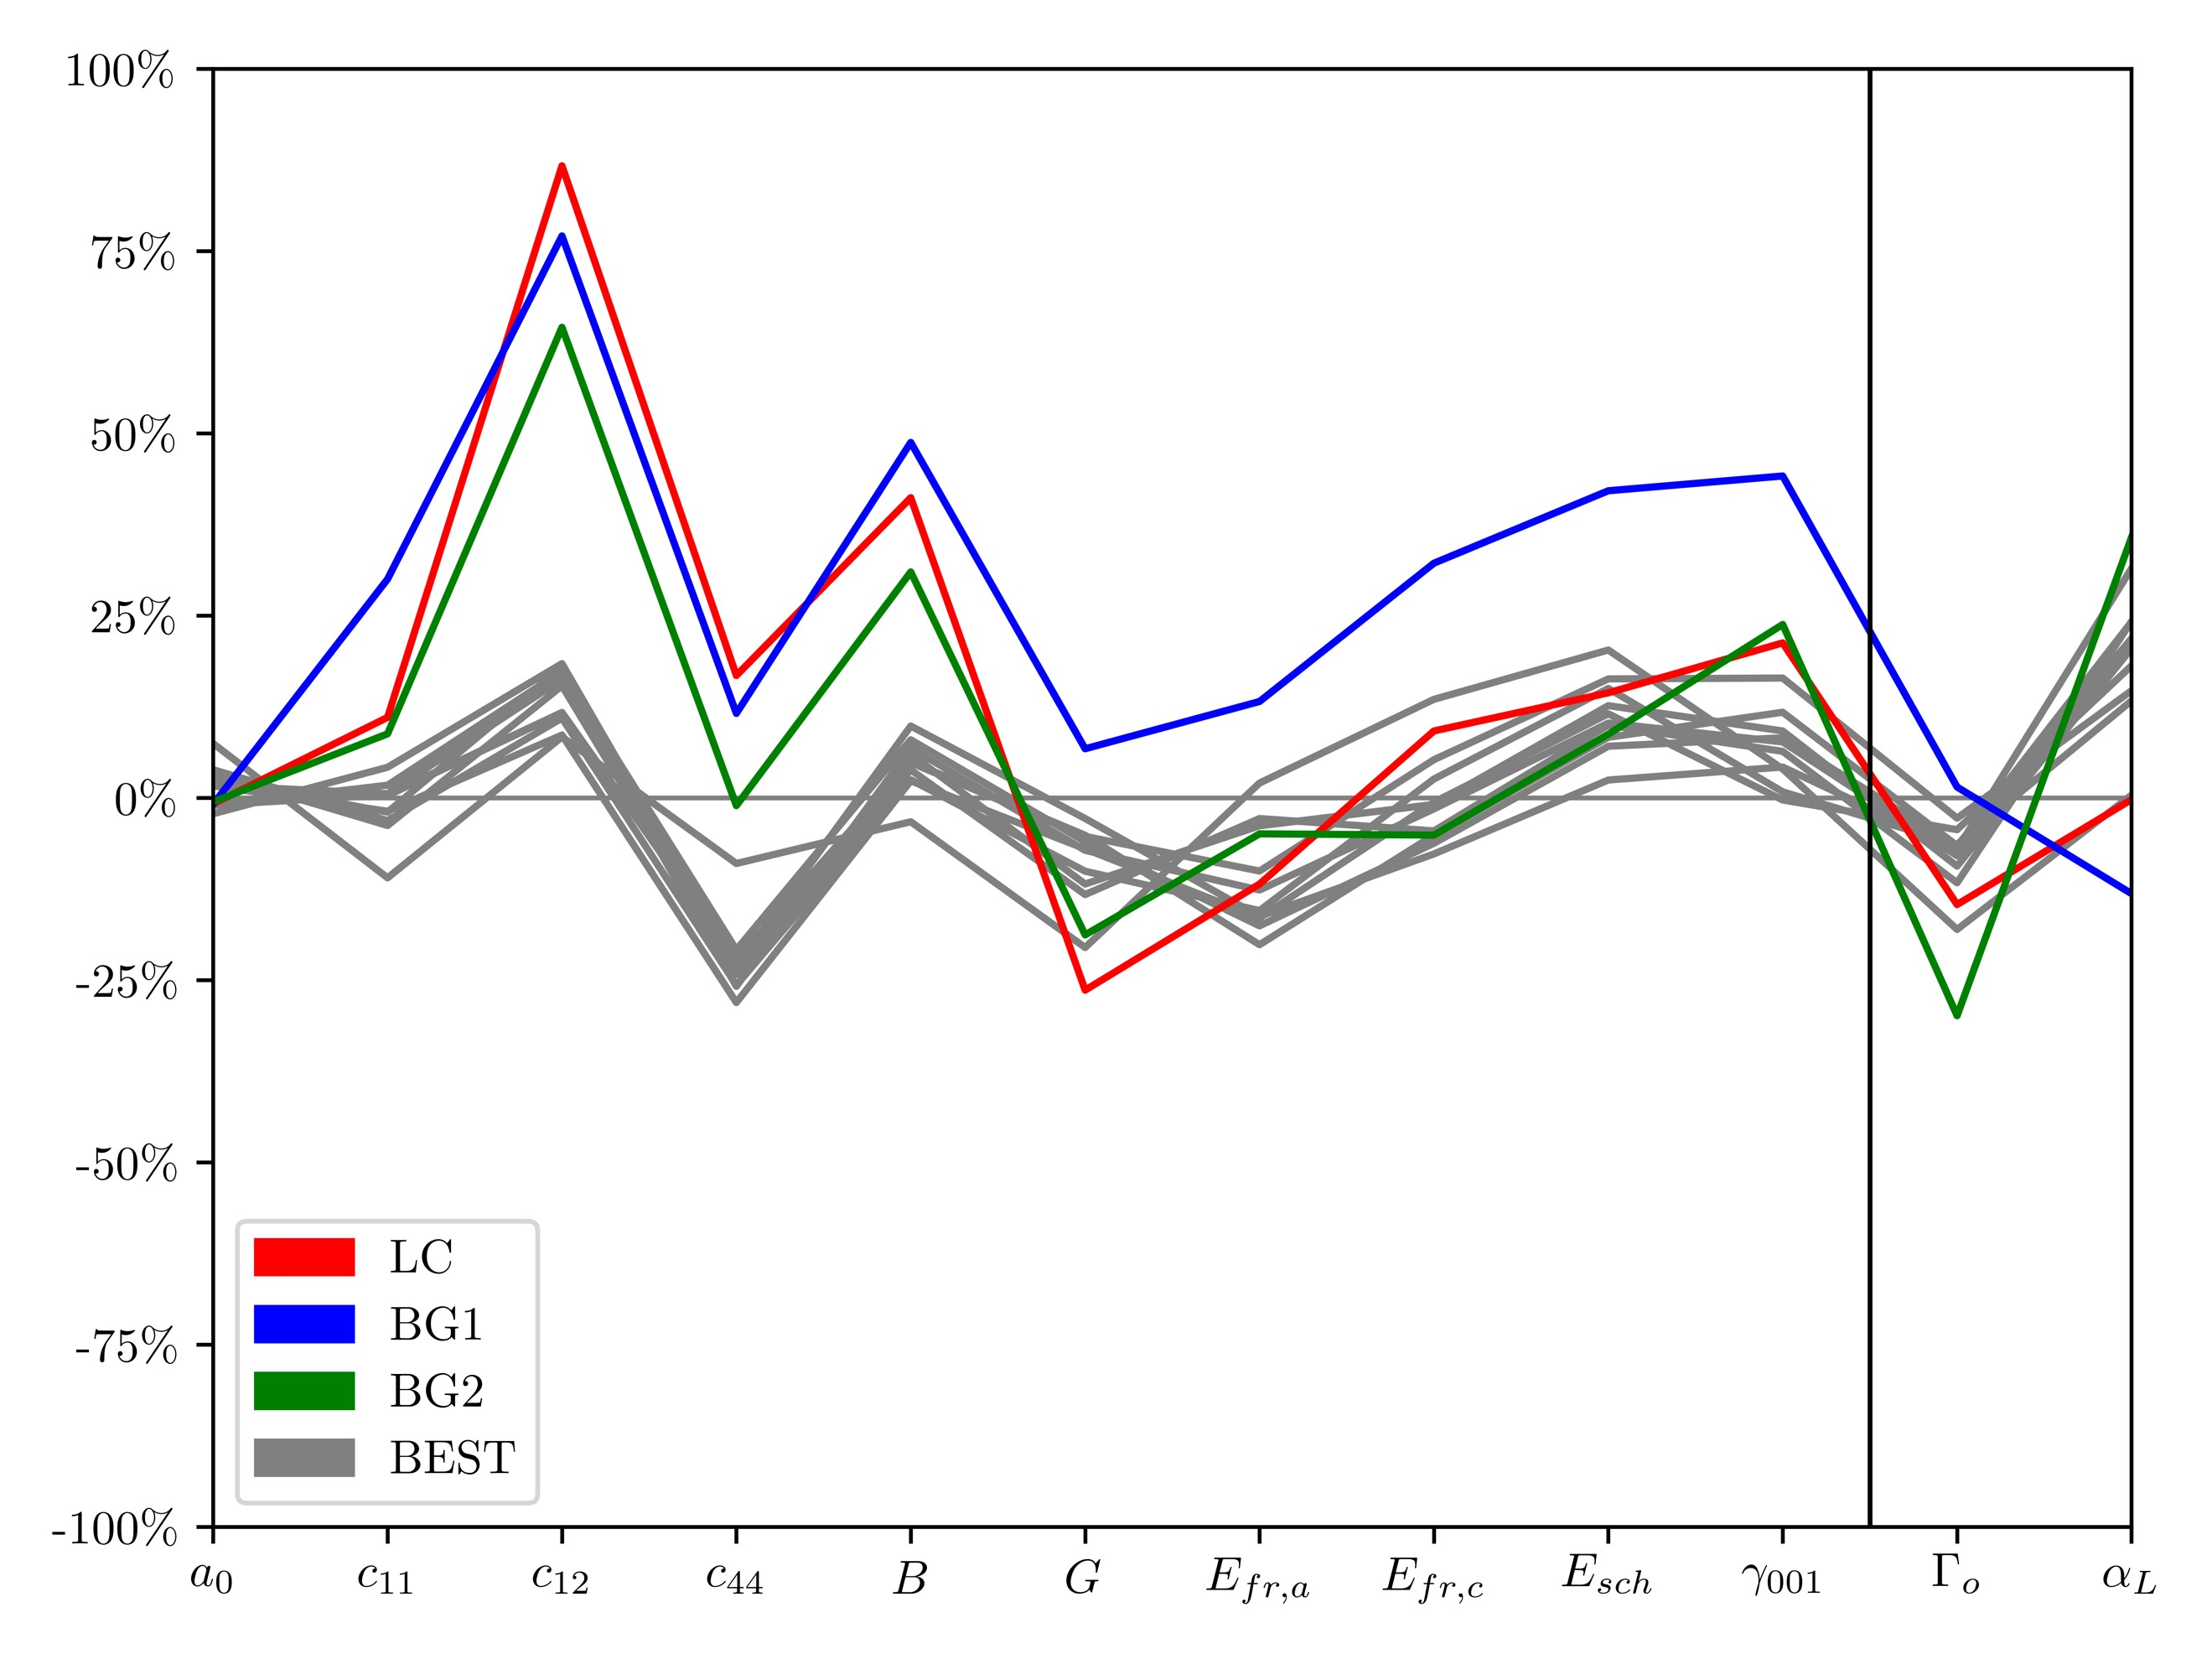
\includegraphics[width=0.8\textwidth]{chapter7/MgO_qoi_parallel_plots}
  \caption{Errors for the 10 best potentials and the LC and two BG potentials with the same labeling as in the previous figure. The overall best potential determined from our Pareto analysis is given the thick gray line. The QOIs to the left of the vertical line are used in the paramterization; those to the right are predictions.}
  \label{fig:MgO_qoi_parallel_plots}
\end{figure}

\begin{table}[ht]
	\caption{Parameters of the the three expert-develop potentials and the 10 potentials, out of 7557 Pareto optimal potentials with the normalized lowest squared errors.}
	\label{tbl:MgO_best_param}
	\centering
	\begin{tabular}{ccccccc}
		\hline
		{sim\_id} & $Z_{\text{Mg}}$ & $A_{\text{Mg-O}}$ & $\rho_{\text{Mg-O}}$ & $A_{\text{O-O}}$ & $\rho_{\text{O-O}}$ * $C_{\text{O-O}}$ \\
    \hline
		LC  & 2.0 & 821.60   & 0.32000 & 22764.00 & 0.14900 & 27.88 \\
		BG1 &	2.0 &	1279.69  &	0.29969 &	9547.96 &	0.21916 &	32.00 \\
		BG2 &	1.7	& 929.69   & 0.29909 & 4870.00 & 0.26700 & 7.00 \\
		550 &	1.6	& 1270.77	 & 0.28993 &	25294.69 & 0.23093 & 64.71 \\
		762  &	1.6	& 1093.66	 & 0.28812 &	27681.46 & 0.19519 & 33.99 \\
		5965 &	1.6	& 1011.10	 & 0.29378 &	15450.62 & 0.20124 & 44.60 \\
		8984 &	1.7	& 1410.19	 & 0.28510 &	27180.53 & 0.06775 & 9.99 \\
		5429 &	1.6 &	1256.22	 & 0.27391 & 8102.88 & 0.22447 & 23.70 \\
		467  &	1.7	& 1257.11	 & 0.28573 & 6737.95 & 0.22696 & 38.30 \\
		5111 &	1.7	& 1248.66	 & 0.29113 & 23232.83 &	0.22658 & 57.45 \\
		3406 &	1.6	& 1217.43	 & 0.29004 & 4426.24 & 0.25216 & 52.18 \\
		2026 &	2.0	& 1038.86	 & 0.33089 & 11256.34 & 0.23727 &	21.60 \\
		2264 &	1.7	& 1291.41	 & 0.29827 & 23242.62 & 0.09337 &22.82 \\
		\hline
	\end{tabular}
\end{table}

\begin{table}[ht]
	\caption{Predicted values of targeted and non-targeted properties for the potential parameters in Table \ref{tbl:MgO_target}}
  \label{tbl:MgO_best_qoi}
	\centering
	\begin{tabular}{ccccccccccc}
		\hline
	  sim\_id &	$a_0$ & $C_{11}$ & $C_{12}$ & $C_{44}$ & $B$ & $G$ &
		          $E_(\text{fr,a})$ & $E_(\text{fr,c})$ & $E_{\text{sch}}$ &
							$\gamma_{\text{\hkl<100>}}$ \\
		        & [\AA] & [GPa] & [GPa] & [GPa] & [GPa] & [GPa] &
						  [eV] & [eV] & [eV] &
							[$\text{eV/\AA}^2$] \\
	  \hline
		LC   & 4.21 & 308 & 171 & 168 & 217 & 68 & 9.68 & 9.81 & 5.80 & 0.068 \\
		BG1  & 4.21 & 360 & 162 & 161 & 228 & 99 & 12.4 & 11.9 & 7.20 & 0.081 \\
		BG2 & 4.22 & 301 & 151 & 142 & 201 & 75 & 10.4 & 8.53 & 5.51 & 0.069 \\
		1550 & 4.39 & 266 & 106 &	109 & 159 & 80 & 10.7 & 8.58 & 5.57 & 0.060 \\
		762 & 4.20 & 282 & 108 & 114 & 166 & 87 & 9.05 & 8.43 & 5.43 & 0.061 \\
		5965 & 4.20 & 278 & 102 & 112 & 161 & 88 & 8.77 & 8.53 & 5.49 & 0.063 \\
		8984 & 4.32 & 272 & 100 & 104 & 157 & 86 & 9.17 & 8.93 & 5.65 & 0.056 \\
		5429 & 4.15 & 289 & 109 & 111 & 169 & 90 & 9.19 & 8.29 & 5.19 & 0.058 \\
		467 & 4.22 & 278 & 102 & 112 & 161 & 88 & 9.89 & 9.46 & 5.89 & 0.065 \\
		5111 & 4.35 & 272 & 108 & 109 & 163 & 82 & 10.6 & 8.91 & 5.71 & 0.061 \\
		3406 & 4.32 & 279 & 107 & 107 & 164 & 86 & 9.59 & 8.85 & 5.59 & 0.060 \\
		2026 & 4.56 & 247 & 99 & 131 & 148 & 74 & 11.2 & 10.2 & 6.09 & 0.058 \\
		2264 & 4.41 & 268 & 102 & 107 & 157 & 83 & 9.28 & 9.22 & 5.83 & 0.056 \\
		\hline
	\end{tabular}
\end{table}

\begin{table}
	\caption{Predicted values of targeted and non-targeted properties for the potential parameters in Table \ref{tbl:MgO_target}}
	\label{tbl:MgO_best_testing_qoi}	\centering
		\begin{tabular}{ccc}
			\hline
		  sim\_id &$\Gamma$ & $\alpha(\times 10{-5})$ \\
			        & [$\text{cm}^{-1}$] & [/K] \\
		  \hline
			LC   & 329  & 1.08 \\
			BG1  & 391	& 0.94 \\
			BG2  & 270  & 1.47 \\
			1550 & 340	& 1.34 \\
			762  & 359  & 1.34 \\
			5965 & 360  & 1.32 \\
			8984 & 368  & 1.28 \\
			5429 & 358	& 1.40 \\
			467  & 374	& 1.24 \\
			5111 & 349  & 1.30 \\
			3406 & 354	& 1.31 \\
			2026 & 316  & 1.08 \\
			2264 & 360  & 1.22 \\
			\hline
		\end{tabular}
\end{table}

\section{Discussion and Conclusions}
This chapter illustrates a method that turns the parameterization of a classical interatomic potential from a largely ill-defined, supervised learning process to a well-defined, unsupervised, machine-learning algorithm.  This new approach frees the potential developer from the need to make a priori assumptions that must be varied iteratively in an ad hoc approach.  By exploiting the concept of Pareto optimality, the potential development process is transformed to one in which the potential developer can select a parameterization \emph{a posteriori} from an ensemble of parameterizations. While the use of a metric which contains the subjective preferences of the potential developer is unavoidable, the process of parameterization within a Pareto framework delays this choice to the end of the potential development process; moreover; the ensemble of Pareto-optimal potentials allows the potential developer to make a choice of acceptable errors that is informed by the actual capabilities of the potential form.

The Pareto approach was presented as an analytical framework that is related to minimization of a weighted cost function which minimizes the weighted square differences. The Pareto surface is the set of all potential optimal parameterizations when the weights of the cost functions are unspecified. This approach provides a mechanism for comparing the performance of different formalisms, understanding the tradeoffs in improving the fidelity of replicating one material property at the expense of the other, and having a mechanism of creating a population of potential parameter sets from which a probability density function can be defined for uncertainty quantification applications.

Finally, this approach was motivated by the need for an algorithmic potential development process that can act as the foundation for systematic uncertainty quantification. It is clear that the ensemble of Pareto-optimal potentials provides a rich database that can be analyzed in multiple ways and can be the basis for uncertainty quantification.
